\usetikzlibrary{arrows.meta,calc,matrix,positioning,shapes.multipart}

\begin{frame}[fragile,label=vm]{recall(?): virtual memory}
\begin{itemize}
\item illuision of \myemph{dedicated memory}
\end{itemize}
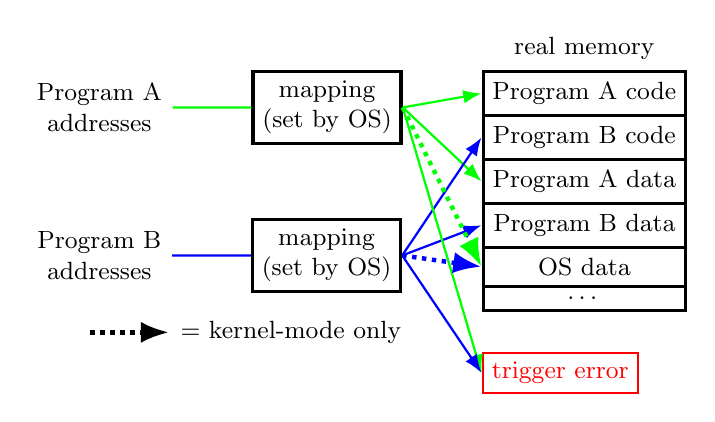
\begin{tikzpicture}
\tikzset{
    every node/.style={font=\small},
}
\node[align=center] (progAAddr) {Program A \\ addresses};
\node[below=1cm of progAAddr,align=center] (progBAddr) {Program B \\ addresses};
\node[draw, right=1cm of progAAddr,align=center] (translationA) { mapping \\ (set by OS) };
\node[draw, right=1cm of progBAddr,align=center] (translationB) { mapping \\ (set by OS) };
\node[draw,rectangle split, rectangle split parts=6, anchor=north west,label={north:real memory}] (mem) at ([xshift=1cm]translationA.north east) {
    \nodepart{one}
    Program A code 
    \nodepart{two}
    Program B code
    \nodepart{three}
    Program A data
    \nodepart{four}
    Program B data
    \nodepart{five}
    OS data
    \nodepart{six}
    \ldots
};
\draw[-Latex,green,thick] (progAAddr) -- (translationA) (translationA.east) -- (mem.one west);
\draw[-Latex,green,thick] (translationA.east) -- (mem.three west);
\draw[-Latex,blue,thick] (progBAddr) -- (translationB) (translationB.east) -- (mem.two west);
\draw[-Latex,blue,thick] (translationB.east) -- (mem.four west);
\node[thick,red,draw,anchor=north west] (error) at ([yshift=-.5cm]mem.south west) {trigger error};
\draw[-Latex,green,thick] (translationA.east) -- (error.west);
\draw[-Latex,blue,thick] (translationB.east) -- (error.west);
\draw[-Latex,green,ultra thick,dotted] (translationA.east) -- (mem.five west);
\draw[-Latex,blue,ultra thick,dotted] (translationB.east) -- (mem.five west);
\draw[-Latex,ultra thick,dotted] ([xshift=-3cm,yshift=-.5cm]translationB.south) -- ([xshift=-2cm,yshift=-.5cm]translationB.south)
    node[right] {= kernel-mode only};
\end{tikzpicture}
\end{frame}


\begin{frame}[fragile,label=segmentation]{segmentation}
    \begin{itemize}
    \item before virtual memory, there was \myemph{segmentation}
    \end{itemize}
\begin{tikzpicture}
    \tikzset{>=Latex}
    \node[draw,label={north:address},rectangle split,rectangle split parts=2,
        rectangle split horizontal,font=\small,align=left] (address) {
        segment \#: \\ \color{orange!70!black}{\tt 0x1} \nodepart{two} offset: \\ \color{magenta!70!black}{\tt 0x23456}
    };
    \matrix[tight matrix,nodes={text width=2cm,font=\small\tt,text depth=.4ex,text height=1.2ex},
        column 1/.style={nodes={text width=1.5cm}},
        anchor=north west,
        visible on=<1>,
    ] (table) at ([xshift=.5cm]address.north east){
        seg \# \& base \& limit \\
        0 \& 0x14300 \& 0x60000 \\
        |[orange!70!black]| 1 \& |[blue!70!black]| 0x50000 \& |[green!70!black]| 0x6F000 \\
        2 \& 0x70000 \& 0x30000 \\
    };
    \matrix[tight matrix,nodes={text width=2cm,font=\small\tt,text depth=.4ex,text height=1.2ex},
        column 1/.style={nodes={text width=1.5cm}},
        column 3/.style={nodes={font=\scriptsize\tt, text width=6cm}},
        anchor=north west,
        visible on=<2>,
    ] (table2) at ([xshift=.5cm]address.north east){
        seg \# \& base \& limit \\
        0 \& 0x0 \& 0xFFFF FFFF FFFF FFFF \\
        |[orange!70!black]| 1 \& |[blue!70!black]| 0x0 \& |[green!70!black]| 0xFFFF FFFF FFFF FFFF \\
        2 \& 0x0 \& 0xFFFF FFFF FFFF FFFF \\
    };
    \node[draw,circle,font=\large] (plus) at ([yshift=-2cm]address.two south) { $+$ };
    \node[font=\large,draw] (less) at (table-3-3.south |- plus) { $<=$ };
    \draw[magenta!70!black,thick,->] (address.two south) -- (plus);
    \draw[blue!70!black,thick,->] (table-3-2.south) |- (plus);
    \draw[green!70!black,thick,->] ([xshift=.25cm]table-3-3.south) -- ([xshift=.25cm]less.north);
    \draw[magenta!70!black,thick,->] (address.two south) -- ($(plus.north) + (0, .5cm)$) -| ([xshift=-.25cm]less.north);
    \draw[thick,->] (plus) -- ++ (0,-1cm) node[below] { computed address };
    \draw[thick,->] (less) -- ++ (0,-1cm) node[below,align=center] { no segmentation \\ fault?};
\end{tikzpicture}
\end{frame}


\begin{frame}[fragile, label=x86Seg]{x86 segmentation}
\begin{itemize}
\item addresses you've seen are the \myemph{offsets}
\item but every access uses a segment number!
\item segment numbers come from registers
    \begin{itemize}
    \item CS --- code segment number (jump, call, etc.)
    \item SS --- stack segment number (push, pop, etc.)
    \item DS --- data segment number (mov, add, etc.)
    \item ES --- addt'l data segment (string instructions)
    \item FS, GS --- extra segments (never default)
    \end{itemize}
\item instructions can have a \myemph{segment override}:
\begin{lstlisting}
movq $42, %fs:100(%rsi)
    // move 42 to segment (# in FS),
    // offset 100 + RSI 
\end{lstlisting}
\end{itemize}
\end{frame}

\begin{frame}[fragile,label=x86SegPic]
\vspace{-.25cm}
\tikzset{every picture/.style={very thick},every node/.style={fill=white,inner sep=.1mm}}
\begin{tikzpicture}
\node[anchor=north west] at (0,0){
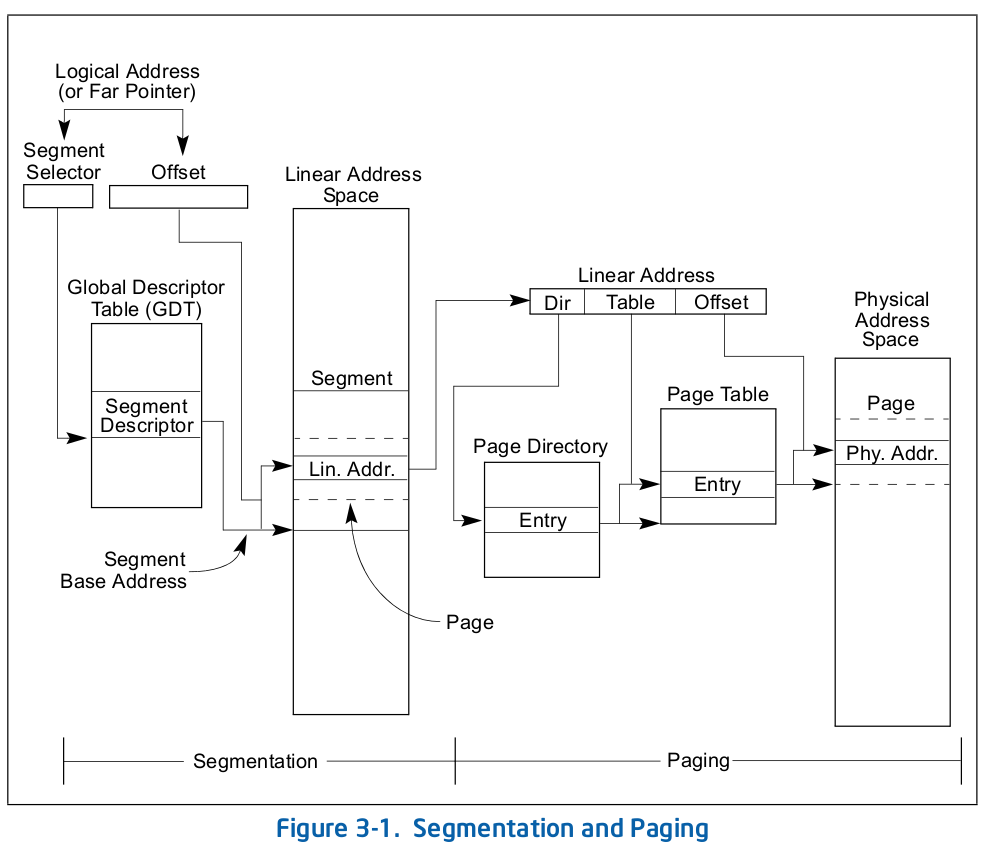
\includegraphics[width=0.78\textwidth]{../asm/seg-and-page}
};
%\draw[help lines] (0,0) grid (12, -8);
\begin{visibleenv}<2>
    \draw[blue] (0.8,-0.8) rectangle (2.5,-1.4);
    \node[text=blue!70!black,anchor=south,font=\small] at (1.6,-.8) {program address};
    \draw[green] (6.4,-3.3) rectangle (9.1,-3.9);
    \node[text=green!70!black,anchor=south,font=\small,align=center] at (7.5,-3.3) {after segmentation \\
                                                  ``virtual address''};
    \draw[magenta] (0.9,-3.4) rectangle (2.8,-6.1);
    \node[text=magenta!70!black,anchor=south,font=\small] at (1.8,-3.4) {segment table};
\end{visibleenv}
\begin{visibleenv}<3>
    \draw[red] (0.3,-1.6) rectangle (1.4,-2.4);
    \node[text=red,anchor=west] at (1.4,-2.0) {from instruction + segment register};
\end{visibleenv}
\end{tikzpicture}
\imagecredit{Figure: Intel manuals, Vol 3A}
\end{frame}

\begin{frame}{x86 segment descriptor}
\vspace{-.25cm}
\tikzset{every picture/.style={very thick},every node/.style={fill=white,inner sep=.2mm}}
\begin{tikzpicture}
\node[anchor=north west] at (0,0){
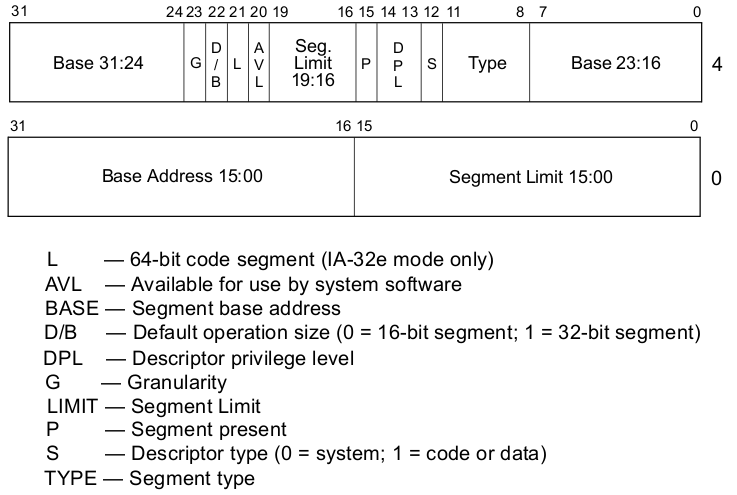
\includegraphics[width=0.78\textwidth]{../asm/segment-descr}
};
%\draw[help lines] (0,0) grid (12, -8);
\begin{visibleenv}<2>
\draw[draw=red] (0.6, -5.4) rectangle (5.8, -5.8) node[right,text=red] {
    user or kernel mode? (if code)
};
\end{visibleenv}
\begin{visibleenv}<3>
\draw[draw=red] (0.6, -3.9) rectangle (8.0, -4.3);
\draw[draw=red] (0.6, -5.0) rectangle (11.0, -5.4);
\node[draw=red,text=red!60!black,anchor=north] at (5.0, -5.6) {
    64-bit or 32-bit or 16-bit mode? (if code)
};
\end{visibleenv}
\end{tikzpicture}
\imagecredit{Figure: Intel manuals, Volume 3A}
\end{frame}


\begin{frame}{64-bit segmentation}
\begin{itemize}
\item in 64-bit mode:
\item limits are ignored
\item base addresses are ignored
\item \ldots except for {\tt \%fs}, {\tt \%gs}
    \begin{itemize}
    \item when explicit segment override is used
    \end{itemize}
\item effectively: extra pointer register
\end{itemize}
\end{frame}


